% In-paper appendix C: calibration disclosure (was appendix D.3; kept in
% the paper for integrity per the editorial memo / decision stub D305
% recommendation; content unchanged).

\rb{K}{APC-01}{The full audit trail for the band scale, including the excluded test-selected value quoted only here. Integrity material that must stay in the paper.}The forecast-derived filter's band scale carries a full audit trail. The
production value $c = 1.77$ is the coverage calibration of
\S\ref{sec:methods_rexenkf}, selected on validation before any test encounter
was seen. During exploration a band of $c = 4$ was evaluated against
the \TestSplit{} set and reached \PoneExcludedBandFour{} impact median there; because
that value was selected with the test split in view, it is excluded from
every table and headline of this paper and quoted only here. The
consistency calibration (grid and rule committed before
any value was seen) subsequently showed that the innovation statistic
rejects large bands on held-out training encounters even though their
tracking is better (\S\ref{sec:res_da}): the large-band gain is real and
reproducible on encounters never used for selection, but it is model-error
compensation, not calibration, and the paper's route, selected without reference to the test set, to
comparable performance is the \TwoStageKF{} instead. The \TwoStageKF{}
run at the coverage band was itself declared in the pre-registration
record after the consistency-selected run was seen and before any run at
the declared configuration existed; both frozen runs are reported in
\S\ref{sec:res_da} regardless of outcome, and the declaration order ships
with the data record.\re

% Moved out of Methods \S3.4 on Carlos's 2026-08-13 comment on S34-06: a textbook
% recursion whose result is three sentences in \S4.6.3. It sits here rather than
% in appendix A because the figure below already carries the smoother comparison,
% so the recursion and its result are now on the same page. \S3.4 keeps the
% one-sentence form and points at app:rts.
\subsubsection*{The fixed-lag smoother}
\label{app:rts}

\rb{K}{APC-02}{The fixed-lag recursion, moved out of \S3.4. Its result is three sentences in \S4.6.3, and the figure below already carries the smoother comparison.}The reanalysis reference of \S\ref{sec:methods_rexenkf} is a fixed-lag
Rauch--Tung--Striebel smoother running on the linear stack of
\S\ref{sec:methods_lae}. A filter reports the best estimate available from
pressure up to the present frame; a smoother goes back and revises that estimate
once a few later frames have arrived, which is legitimate whenever the
application can tolerate the delay. Writing $(\zvec^{f}_k, P^{f}_k)$ and
$(\zvec^{a}_k, P^{a}_k)$ for the forecast and analysis moments from the forward
Kalman pass, the backward recursion over the lag window is
\begin{equation}
  C_k = P^{a}_k A^{\mathsf{T}} \left(P^{f}_{k+1}\right)^{-1},
  \qquad
  \zvec^{s}_k = \zvec^{a}_k + C_k\left(\zvec^{s}_{k+1} -
  \zvec^{f}_{k+1}\right),
  \label{eq:rts}
\end{equation}
in which $C_k$ weights how much of the later smoothed estimate to propagate
back, large where the forward analysis was uncertain relative to the forecast it
led to. We apply it over a lag of $L = 5$ frames, a fixed reporting latency of
$0.25\,c/u_\infty$: the smoothed estimate at $t$ uses pressure up to $t + L$ and
nothing later, so it remains causal at that delay. The ensemble smoother variant
on the \FnoiseKF{}, a lagged cross-covariance update of the stored member
history, degrades the filter and is reported as a negative in the supplementary
material.\re

% Moved from Results (Session 39 figure pass, D-B): the estimator-ladder, smoother
% and NIS-calibration panels split off the main-text tracking figure.
\begin{figure}
  \centering
  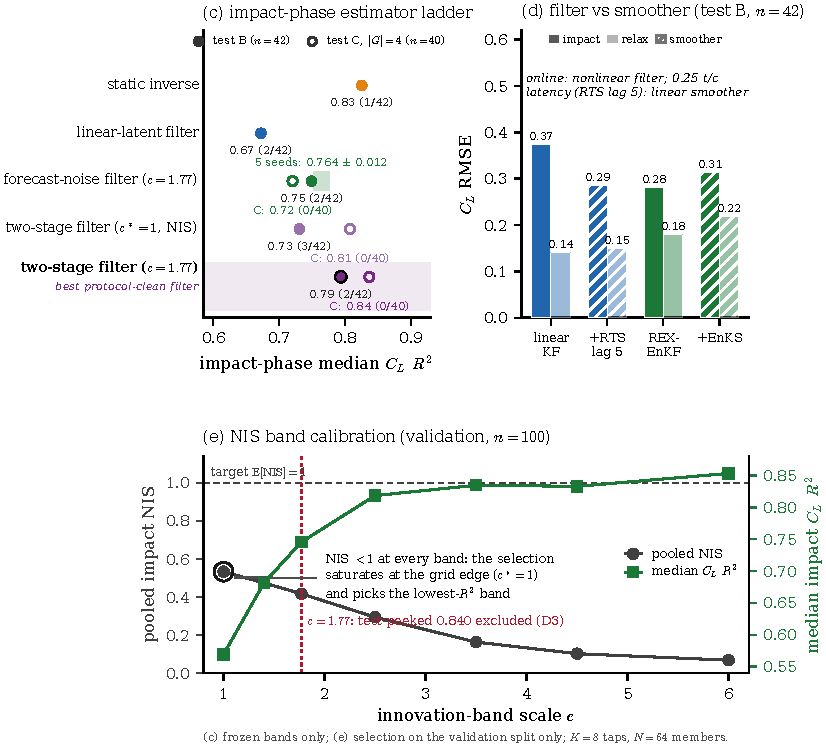
\includegraphics[width=0.82\linewidth]{sections/figures/results/fig_da_calibration_v4.pdf}
  \caption{\rb{K}{APC-C1}{The estimator ladder, the smoother comparison and the band calibration in one figure. Carries the static-inverse claim the abstract makes.}Estimator calibration and selection (\TestSplit, \ValSplit{} and,
  through the open markers, \BoundarySplit{}
  sets; parenthetical counts on the ladder are large-error encounters,
  impact-phase $R^2 < -1$, per set). (a) The impact-phase estimator ladder with
  the five-seed
  member-noise band, open markers the frozen \BoundarySplit{} values; (b)
  the filter against the fixed-lag smoother; (c) the band-scale calibration
  on the held-out training encounters, where innovation consistency and tracking
  disagree and the selection saturates at the grid edge.\re}
  \label{fig:calibration}
\end{figure}
